\documentclass[12pt, titlepage]{article}
\usepackage{beamerarticle}
\usepackage[utf8]{inputenc}
\usepackage{amssymb,amsmath}

% Page settings
\usepackage[left=1in, right=2in, top=1in, bottom=1in]{geometry}
\usepackage{times} % palatino, lmodern
\usepackage{setspace}
\onehalfspacing
%\doublespacing  % \singlespacing 

% Appendix
\usepackage{appendix}

% Figure caption on top
% See: https://github.com/axelsommerfeldt/caption/blob/master/doc/caption-eng.pdf
\usepackage[bf,textfont=sc,figureposition=top,tableposition=top]{caption}

% Line numbers
%\usepackage{lineno}+
%\linenumbers

% Links
\usepackage{hyperref}
\hypersetup{%
  colorlinks=false,% hyperlinks will be black
  linkbordercolor=red,% hyperlink borders will be red
  pdfborderstyle={/S/U/W 1}% border style will be underline of width 1pt
}

% Tables
\usepackage{array,booktabs,longtable,rotating}

% Position tables {here, top, bottom, page}
\makeatletter
\def\fps@table{htbp}
\makeatother

%% ... at the end of paper

% Create new minipage environment for notes 
% at the bottom of tables or figures
\newenvironment{tablenotes}[1][Note:]{
  \vskip 1.8ex
  \begin{minipage}{\textwidth}\itshape\footnotesize{#1}
} {\end{minipage}}


% Graphics
\usepackage{graphicx,grffile}
\makeatletter
\def\maxwidth{\ifdim\Gin@nat@width>\linewidth\linewidth\else\Gin@nat@width\fi}
\def\maxheight{\ifdim\Gin@nat@height>\textheight\textheight\else\Gin@nat@height\fi}
\makeatother
% Scale images if necessary, so that they will not overflow the page
% margins by default, and it is still possible to overwrite the defaults
% using explicit options in \includegraphics[width, height, ...]{}
\setkeys{Gin}{width=\maxwidth,height=\maxheight,keepaspectratio}
% set default figure placement to htbp
\makeatletter
\def\fps@figure{htbp}
\makeatother

\usepackage{natbib}% plainnat
\bibliographystyle{abbrvnat}
\setcitestyle{authoryear,open={(},close={)}}
%\bibliographystyle{aer}


\setlength{\emergencystretch}{3em}  % prevent overfull lines
\providecommand{\tightlist}{%
  \setlength{\itemsep}{0pt}\setlength{\parskip}{0pt}}


\usepackage{todonotes}

\title{Incentives for Public Goods Inside Organizations: Field Experimental
Evidence\thanks{Blasco: Harvard Institute for Quantitative Social Science, Harvard
University, 1737 Cambridge Street, Cambridge, MA 02138 (email:
\href{mailto:ablasco@fas.harvard.edu}{\nolinkurl{ablasco@fas.harvard.edu}}).
Jung: Harvard Business School, Soldiers Field, Boston, MA 02163 (email:
\href{mailto:oliviajung@gmail.com}{\nolinkurl{oliviajung@gmail.com}}),
Lakhani: Harvard Business School, Soldiers Field, Boston, MA 02163, and
National Bureau of Economic Research (email:
\href{mailto:k@hbs.edu}{\nolinkurl{k@hbs.edu}}). Menietti: Harvard
Institute for Quantitative Social Science, Harvard University, 1737
Cambridge Street, Cambridge, MA 02138 (email:
\href{mailto:mmenietti@fas.harvard.edu}{\nolinkurl{mmenietti@fas.harvard.edu}}).
We gratefully acknowledge the financial support of the MacArthur
Foundation (Opening Governance Network), NASA Tournament Lab, and the
Harvard Business School Division of Faculty Research and Development.
This project would not have been possible without the support of Eric
Isselbacher, Julia Jackson, Maulik Majmudar and Perry Band from the
Massachusetts General Hospital's Healthcare Transformation Lab.}}
\author{Andrea Blasco \and Olivia S. Jung \and Karim R. Lakhani \and Michael Menietti}
\date{Last updated: 06 December, 2017}

\begin{document}
\maketitle
\begin{abstract}
We report results of a natural field experiment conducted at a medical
organization that sought contribution of public goods (i.e., projects
for organizational improvement) from its 1200 employees. Offering a
prize for winning submissions boosted participation by 85 percent
without affecting the quality of the submissions. The effect was
consistent across gender and job type. We posit that the allure of a
prize, in combination with mission-oriented preferences, drove
participation. Using a simple model, we estimate that these preferences
explain about a third of the magnitude of the effect. We also find that
these results were sensitive to the solicited person's gender.

\smallskip\noindent 
JEL Classification: D23; H41; M52.

\smallskip\noindent 
Keywords: innovation contest; free rider problem; social preferences; altruism; idea generation; organization of work.
\end{abstract}


\clearpage
\tableofcontents
\setcounter{tocdepth}{2}
\clearpage

\clearpage

\section{Results}\label{results}

\subsection{Submitting project
proposals}\label{submitting-project-proposals}

We first examine treatment differences in participation by looking at
the percentage of employees who made a project submission (Figure
\ref{figure_participation}). Based on the results of the four-week
submission period, we find that, when the solicitation highlights the
opportunity of a prize to be won (PRIZE), employee participation is
considerably higher relative to the other solicitation treatments. In
particular, the proportion of submissions in the PRIZE solicitation
treatment is 7.4 percent, which is 7.4/4.5=1.64 and 7.4/5.2=1.42 times
higher relative to those associated with solicitation treatments
replacing the prize opportunity by a general encouragement to
participate (PCARE, 4.5 percent; and WPLACE, 5.2 percent). The
difference is even more dramatic when the prize opportunity is replaced
by information about available project implementation funding (FUND, 2.3
percent), compared to which the proportion of submissions in the PRIZE
solicitation treatment is 7.4/2.3=3.22 times higher.

\begin{figure}
\caption{Employee participation by solicitation treatment}
\label{figure_participation}
\centering
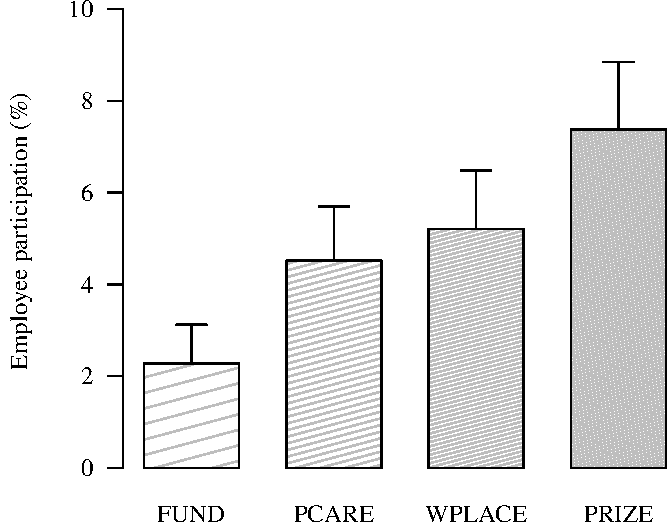
\includegraphics{figures/figure_participation-1.pdf}
\end{figure}

\begin{table}
\centering
\caption{Pairwise difference in participation rates}
\label{pairwise}
\begin{tabular}{@{}lccc}
  \\[-1.8ex]\hline \hline \\[-1.8ex]
 & Lower & Upper & P-value \\ 
  \hline \\[-1.86ex]
PRIZE - FUND & 1.756 & 8.442 & 0.003 \\ 
  PRIZE - PCARE & -0.853 & 6.564 & 0.132 \\ 
  PRIZE - WPLACE & -1.659 & 5.980 & 0.269 \\ 
  FUND - PCARE & -5.092 & 0.605 & 0.124 \\ 
  FUND - WPLACE & -5.931 & 0.053 & 0.055 \\ 
  PCARE - WPLACE & -4.090 & 2.699 & 0.688 \\ 
   \\[-1.8ex]\hline \hline \\[-1.8ex]
\end{tabular}
\begin{tablenotes}
This table reports Wald confidence intervals (95 percent level) for the difference in the proportions of submissions between every two solicitation treatments. The last column reports p-values from a two-sided proportion test where the null tested is that, for a given pair, the proportions of submissions in each group are equal.
\end{tablenotes}
\end{table}

To test to see whether participation rates are statistically different
across solicitation treatments, we use a series of pairwise two-sample
tests of proportions (Table \ref{pairwise}). The analysis reveals that
the positive difference between the PRIZE and PCARE solicitation
treatments is marginally statistically significant (p=0.132); the
positive difference between the PRIZE and WPLACE solicitation treatments
is insignificant (p=0.269); and the positive difference between the
PRIZE and FUND solicitation treatments is statistically significant
(p=0.003). This evidence thus indicates a positive causal effect on
participation of highlighting the prize opportunity compared to a
general encouragement (although only marginally significant) and
announcing available funding.

The analysis of the pairwise comparisons shows further a negative
difference between the FUND and the WPLACE solicitation treatments that
is statistically significant (p=0.055); and a negative difference
between the FUND and the PCARE solicitation treatments that is
marginally statistically significant (p=0.124). This evidence thus
indicates a negative causal effect on employee participation of
highlighting the available funding compared to a general encouragement
to participate. In other words, while a solicitation strategy based on
individual prizes is effective, a solicitation focused on the
opportunity of getting implementation funding alone could harm
participation relative not only to prizes but also to general
encouragements towards improving the workplace.

\begin{figure}
\caption{Submissions over time by solicitation treatment}
\label{figure_dynamics}\centering
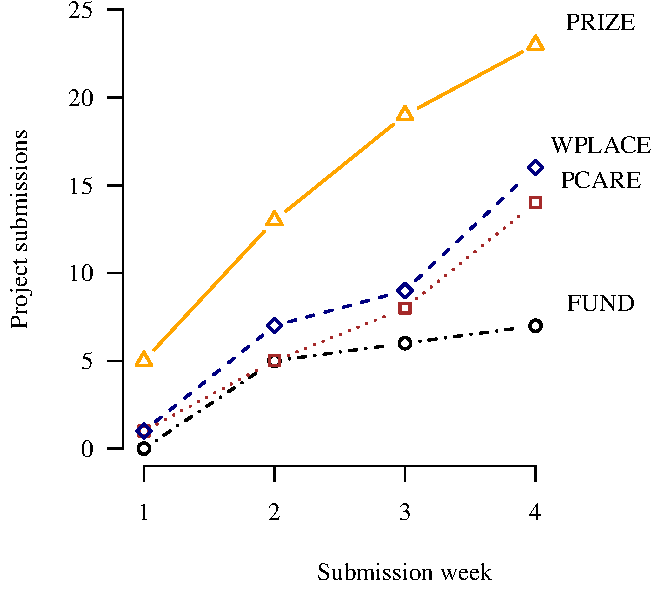
\includegraphics{figures/figure_dynamics-1.pdf}
\end{figure}

We now turn to examining how employee participation evolves over time
(Figure \ref{figure_dynamics}). Though our data may not allow for a
complete analysis of submission dynamics, looking at the overall
submission patterns can be useful for various reasons. In particular, if
employees assigned to different solicitation treatments were sharing
(either face-to-face or electronically) the content of their
solicitation with others, one should expect their participation rates to
converge over time, yielding estimates of the causal effects of a
solicitation treatment biased towards zero. Contrary to these
expectations, Figure \ref{figure_dynamics} shows no evidence of a strong
convergence. Submissions in the PRIZE solicitation treatment are
constantly higher than in the other treatments (except perhaps in the
final week); and, at the same time, submissions in the FUND treatment
are constantly low. These patterns are hence consistent with
communication effects having little, or no, consequences on our
findings, a topic we will discuss in greater detail later (Section
\ref{discussion}).

Another important question related to employee participation is the role
of employee heterogeneity --- i.e., in the benefits from organizational
improvements and the opportunity cost of contributing time and effort.
We, hence, employ a simple regression model to check whether differences
in participation can be explained by differences in the gender,
profession, and organizational role of the employee. The probability of
submitting, \(y_i=1\), is given by

\begin{equation} 
  \label{eq: submit}
    \Pr(y_i=1) = \alpha_0 + \sum_{j} \alpha_{j} \text{SOLICIT}_{ij}
                                    + \text{JOB}_{i} 
                                    + \text{MALE}_{i} 
                                    + \text{OFFICE}_{i}, 
\end{equation}

where \(\alpha_0\) is a constant, \(\alpha_j\) is the causal effect of
the solicitation treatment \(j\) assigned to an employee \(i\)
(\(\text{SOLICIT}_{ij}\)), controlling for the employee's profession
(\(\text{JOB}_i\)), the gender (\(\text{MALE}_i\)), and a dummy for
office location (\(\text{OFFICE}_i\)) that indicates whether the
employee had a permanent office instead of being assigned to a ward.
Note that, in our context, having a fixed office location is highly
correlated with the type of profession.\footnote{Much of the clinical
  staff might be mobile and only half of the employees (\(53\) percent)
  had fixed office locations, as they may be on duty in multiple wards.
  More senior staff tend to have a fixed location. So, within each
  profession, this measure can be viewed as a proxy for status inside
  the organization.} For example, nurses are more likely to being
assigned to a ward than physicians or administrative workers, due to the
nature of their job. Within each profession, however, having a fixed
office location is usually correlated with the hierarchical position
inside the organization. Beyond having a fixed office location per se,
this variable is hence potentially controlling for income and
hierarchical differences occurring within each profession as well.

\begin{table}
\centering
\caption{Probability of submitting proposals}\label{participation ols}
\begin{tabular}{@{\extracolsep{5pt}}lccccc} 
\\[-1.8ex]\hline 
\hline \\[-1.8ex] 
 & \multicolumn{5}{c}{\textit{Dependent variable:}} \\ 
\cline{2-6} 
\\[-1.8ex] & \multicolumn{5}{c}{ $SUBMIT_{ij}=1$ } \\ 
\\[-1.8ex] & (1) & (2) & (3) & (4) & (5)\\ 
\hline \\[-1.8ex] 
 PRIZE & 2.53$^{**}$ & 2.53$^{**}$ & 2.52$^{**}$ & 2.46$^{**}$ & 2.45$^{**}$ \\ 
  & (1.21) & (1.21) & (1.21) & (1.21) & (1.21) \\ 
  & & & & & \\ 
 WPLACE & 0.37 & 0.37 & 0.35 & 0.38 & 0.30 \\ 
  & (1.09) & (1.09) & (1.10) & (1.09) & (1.10) \\ 
  & & & & & \\ 
 FUND & $-$2.57$^{***}$ & $-$2.57$^{***}$ & $-$2.55$^{***}$ & $-$2.49$^{***}$ & $-$2.38$^{***}$ \\ 
  & (0.86) & (0.86) & (0.85) & (0.86) & (0.85) \\ 
  & & & & & \\ 
 Job (nursing) &  & 0.14 &  &  & 1.85 \\ 
  &  & (0.82) &  &  & (1.23) \\ 
  & & & & & \\ 
 Job (MD) &  & $-$0.31 &  &  & $-$1.14 \\ 
  &  & (1.03) &  &  & (1.24) \\ 
  & & & & & \\ 
 Male (yes) &  &  & $-$0.54 &  & $-$0.42 \\ 
  &  &  & (1.33) &  & (1.64) \\ 
  & & & & & \\ 
 Office (yes) &  &  &  & 2.79$^{**}$ & 4.56$^{***}$ \\ 
  &  &  &  & (1.20) & (1.60) \\ 
  & & & & & \\ 
 Constant & 4.84$^{***}$ & 4.78$^{***}$ & 5.00$^{***}$ & 3.35$^{***}$ & 1.97 \\ 
  & (0.61) & (0.66) & (0.73) & (0.75) & (1.25) \\ 
  & & & & & \\ 
\hline \\[-1.8ex] 
Log Likelihood & -5545 & -5545 & -5545 & -5542 & -5540 \\ 
Observations & 1,237 & 1,237 & 1,237 & 1,237 & 1,237 \\ 
\hline 
\hline \\[-1.8ex] 
\end{tabular} 
\begin{minipage}{\textwidth}
\emph{Note:} This table reports OLS estimates with heteroskedasticity robust standard errors in parenthesis. All coefficients are multiplied by 100 to indicate the percentage point change in the probability of submitting. Solicitation treatment dummies are coded to indicate deviations from the overall probability of submitting. The asterisks $^{\ast\ast\ast}$, $^{\ast\ast}$, $^{\ast}$ indicate significance at 1, 5 and 10 percent level, respectively.
\end{minipage}\end{table}

The regression results (Table \ref{participation ols}) show an
insignificant effect on participation associated with an employee's
profession or gender.\footnote{The coefficient for nurses is positive
  and negative for physicians, consistent with sorting. These effects
  are, however, not statistically different from the residual category
  of other workers, as well as from one another.} By contrast, we find a
positive effect associated with the worker having a fixed office
location, as opposed to being assigned to a ward (and the effect size
doubles after controlling for the profession and gender). This evidence
suggests that differences in the employee's hierarchical position inside
the organization, as captured by our office-location regressor, may be a
stronger driver of participation relative to differences in gender and
profession as sometimes assumed by the literature.

The results of the regression model above (Table
\ref{participation ols}) give estimates of the solicitation treatment
differences relative to the overall mean participation and controlling
for baseline characteristics. In theory, these estimates should be more
statistically efficient relative to the pairwise comparisons above
(i.e., by reducing the overall noise associated with baseline
characteristics). We find that, at the 95 level of statistical
significance, employees in the PRIZE solicitation treatment are 2.4
percentage points \emph{more} likely to submit compared to the overall
mean, whereas employees in the FUND solicitation treatment are 2.4
percentage points \emph{less} likely to do so.\footnote{Subtracting
  these two effects gives 4.8 which is the difference in the probability
  of submitting between PRIZE and FUND treatments.} Overall, these
effects are sizable not only in absolute levels but also relative to the
effects of the heterogeneity captured by the other variables.

We now turn to examining treatment interactions involving the employee's
gender and profession (Figure \ref{interactions}).\footnote{We find no
  significant differences for interactions with office location, which
  we do not report for space limitation.} We hypothesize gender
interactions to occur as a result of three main factors: differences in
risk taking, social preferences (willingness to contribute to public
goods), and competitive inclinations. If women prefer to work on
activities that are less risky, more pro-social (e.g., aiming at
improving people's health) and where competition is less intense, then
we should observe significant treatment interactions. Similarly, we
expect treatment interactions associated with the employee's profession
to occur because, for example, the prize opportunity (i.e., the PRIZE
treatment) could be relatively less effective for employees with a
higher income, such as doctors, than the others.

\begin{figure} 
\caption{Employee participation by gender or profession and solicitation treatment}
  \label{interactions}
  \centering
  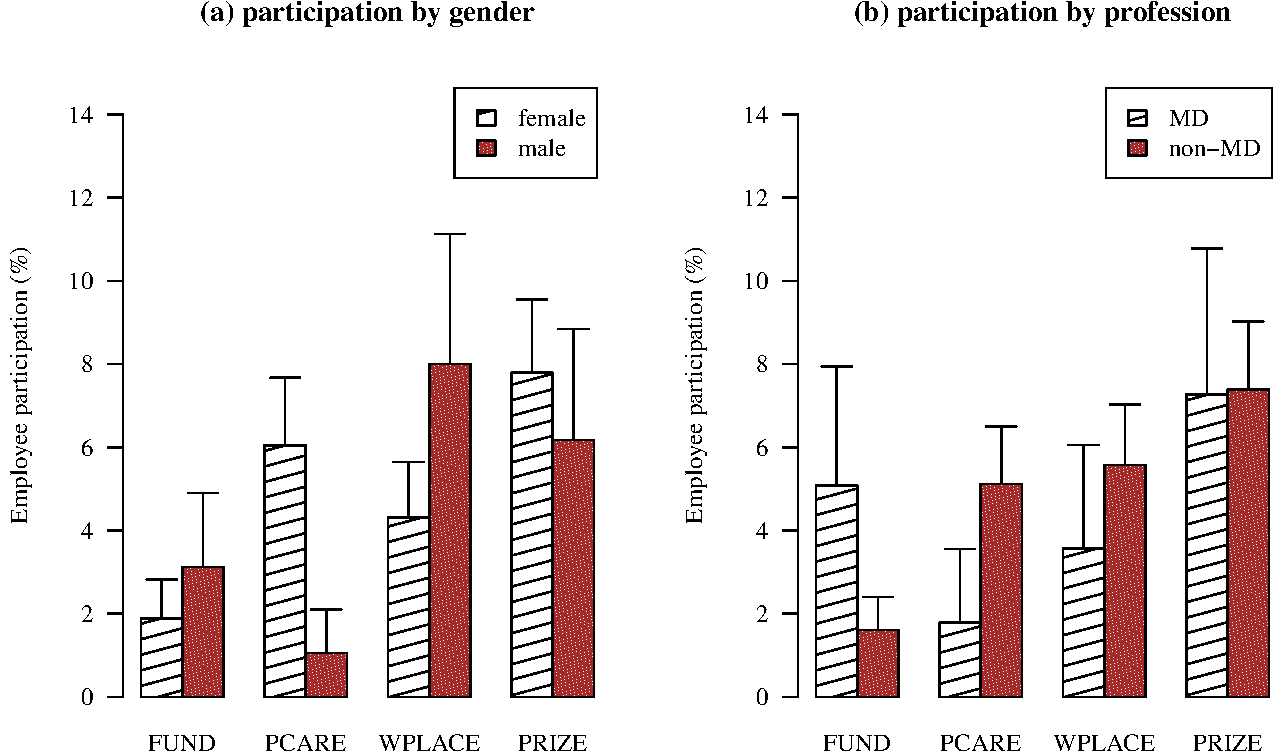
\includegraphics{figures/figure_interactions-1.pdf}
\end{figure}

Examining the proportion of submissions conditional on the gender
(Figure \ref{interactions}, panel a) shows that women are more likely
(about 5 percentage points) to participate than men in the PCARE
solicitation treatment. And examining the same proportion conditional on
the profession (Figure \ref{interactions}, panel b) shows instead that
doctors are as likely to submit as any other worker in PRIZE
solicitation treatment; thus suggesting little sorting based on income
or other characteristics associated with a given profession.

To isolate gender and profession effects, we employ a version of model
\eqref{eq: submit} with gender-treatment interactions.\footnote{We also
  run a model with profession-treatment interactions and results are
  simular to those shown in Figure \ref{fig: interactions}.} The
regression results (Table
\ref{tab: probability submitting interactions}) show similar results to
the simple comparison of proportions. That is, after gradually adding
profession and office controls, interaction coefficients remain stable
across all specifications: the response of men under the PCARE
solicitation treatment is about 3 times the magnitude and in the
opposite direction of the women's response. By subtracting these two
coefficients, we find a significant difference between men and women of
about 5 percentage points (\(p=.018\)), which is consistent with our
previous analysis. Thus, and overall, men respond less than women in the
PCARE solicitation treatment, controlling for the profession and office
location. This effect could be due to gender differences in preferences,
as suggested by the literature, and we will return on this topic in the
discussion of the results.

\begin{table}
\centering
\caption{Gender differences}\label{tab: probability submitting interactions}
\begin{tabular}{@{\extracolsep{5pt}}lccc} 
\\[-1.8ex]\hline 
\hline \\[-1.8ex] 
 & \multicolumn{3}{c}{\textit{Dependent variable:}} \\ 
\cline{2-4} 
\\[-1.8ex] & \multicolumn{3}{c}{ $SUBMIT_{ij}=1$ } \\ 
\\[-1.8ex] & (1) & (2) & (3)\\ 
\hline \\[-1.8ex] 
 PRIZE$\times$female & 2.99$^{*}$ & 2.95$^{*}$ & 2.84 \\ 
  & (1.68) & (1.79) & (1.78) \\ 
  & & & \\ 
 PCARE$\times$female & 1.25 & 1.21 & 1.08 \\ 
  & (1.57) & (1.61) & (1.61) \\ 
  & & & \\ 
 FUND$\times$female & $-$2.91$^{***}$ & $-$2.95$^{**}$ & $-$2.79$^{**}$ \\ 
  & (1.06) & (1.20) & (1.19) \\ 
  & & & \\ 
 WPLACE$\times$female & $-$0.49 & $-$0.52 & $-$0.62 \\ 
  & (1.35) & (1.44) & (1.43) \\ 
  & & & \\ 
 PRIZE$\times$male & 1.37 & 1.42 & 1.40 \\ 
  & (2.44) & (2.51) & (2.50) \\ 
  & & & \\ 
 PCARE$\times$male & $-$3.75$^{***}$ & $-$3.72$^{***}$ & $-$3.64$^{***}$ \\ 
  & (1.15) & (1.16) & (1.16) \\ 
  & & & \\ 
 FUND$\times$male & $-$1.67 & $-$1.65 & $-$1.48 \\ 
  & (1.70) & (1.65) & (1.66) \\ 
  & & & \\ 
 Constant & 4.80$^{***}$ & 4.79$^{***}$ & 1.87$^{*}$ \\ 
  & (0.69) & (0.70) & (1.10) \\ 
  & & & \\ 
\hline \\[-1.8ex] 
Job & no & yes & yes \\ 
Office & no & no & yes \\ 
Log Likelihood & -5542 & -5542 & -5538 \\ 
Observations & 1,237 & 1,237 & 1,237 \\ 
\hline 
\hline \\[-1.8ex] 
\end{tabular} 
\begin{minipage}{\textwidth}
\emph{Note:} This table reports OLS estimates with heteroskedasticity robust standard errors in parenthesis. All coefficients are multiplied by 100 to indicate the percentage point change in the probability of submitting. Solicitation treatment dummies are coded to indicate deviations from the overall probability of submitting. The asterisks $^{\ast\ast\ast}$, $^{\ast\ast}$, $^{\ast}$ indicate significance at 1, 5 and 10 percent level, respectively.
\end{minipage}\end{table}

\subsection{Rating project proposals}\label{rating-project-proposals}

We now turn to examining the outcomes of the peer evaluation phase that
followed the submission phase of the contest. In this phase, 113 project
proposals ended up being rated by a total of 178 employees (14 percent
of our sample) who volunteered for the task.\footnote{We collected 118
  project proposals in total --- five more than those evaluated. Due to
  a technical problem in uploading the proposals on the website for
  evaluation, five proposals ended up with no ratings. This problem was
  independent of the solicitation treatment of the proponent. A Fisher's
  exact test rejects any association between the missed proposals and
  the solicitation received by its proponent (\(p=.7\)).} Their effort
yielded a total of 12,055 evaluator-proposal pairs, providing a very
sensitive test for differences in project quality across our
solicitation treatments.

\begin{table}
\centering

\begin{tabular}{@{\extracolsep{5pt}}lccccc} 
\\[-1.8ex]\hline 
\hline \\[-1.8ex] 
 & \multicolumn{5}{c}{\textit{Dependent variable:}} \\ 
\cline{2-6} 
\\[-1.8ex] & \multicolumn{5}{c}{num\_voted\_ideas \textgreater  0} \\ 
\\[-1.8ex] & (1) & (2) & (3) & (4) & (5)\\ 
\hline \\[-1.8ex] 
 treatmentPCARE & 4.1 &  &  &  & 3.7 \\ 
  & (2.8) &  &  &  & (2.8) \\ 
  & & & & & \\ 
 treatmentWPLACE & 4.6 &  &  &  & 3.9 \\ 
  & (2.8) &  &  &  & (2.8) \\ 
  & & & & & \\ 
 treatmentPRIZE & 2.1 &  &  &  & 1.4 \\ 
  & (2.7) &  &  &  & (2.7) \\ 
  & & & & & \\ 
 jobMD/Fellow &  & 1.4 &  &  & 2.6 \\ 
  &  & (3.0) &  &  & (3.1) \\ 
  & & & & & \\ 
 jobNursing &  & 0.1 &  &  & 4.7 \\ 
  &  & (2.3) &  &  & (3.0) \\ 
  & & & & & \\ 
 gendermale &  &  & $-$2.0 &  & $-$3.5 \\ 
  &  &  & (2.2) &  & (2.6) \\ 
  & & & & & \\ 
 has\_officeyes &  &  &  & 6.5$^{***}$ & 9.5$^{***}$ \\ 
  &  &  &  & (2.0) & (2.6) \\ 
  & & & & & \\ 
 Constant & 11.7$^{***}$ & 14.1$^{***}$ & 14.9$^{***}$ & 10.9$^{***}$ & 5.1 \\ 
  & (1.8) & (1.8) & (1.2) & (1.3) & (3.4) \\ 
  & & & & & \\ 
\hline \\[-1.8ex] 
Observations & 1,237 & 1,237 & 1,237 & 1,237 & 1,237 \\ 
\hline 
\hline \\[-1.8ex] 
\end{tabular} 
\end{table}

We check with linear regression whether the self-selected sample of
staff rating proposals is representative of the whole organization
(Table \ref{drivers_rating}), or just a subset of staff members. Testing
for statistical significance of the coefficients for the profession,
gender, ond office location shows that the evaluators are broadly
representative of the organization as a whole, albeit with a
significantly higher participation from staff members with an office
location. Furthermore, the lack of statistical significance for the
coefficients of the solicitation treatments shows that participation in
the evaluation phase was somewhat independent from the solicitation
treatment the staff members received in the submission phase.\footnote{One
  may find counterintuitive that there was less (although not
  significant) participation in the evaluation phase from employees in
  the PRIZE than in the other solicitation treatments, given the greater
  participation in the submission phase. This result is, however, not
  unexpected because only 70 percent of employees who made submissions
  resolved to rate proposals as well (we detect no difference in the
  propensity of submitting and rating proposals between the treatments);
  so, even a difference of 2 percentage points in submitting will shrink
  to about 1 percentage point in the rating phase. In other words, we
  expect self-rating to do not affect evaluation much.} Thus, and
overall, the collected ratings appear a profession-wide and gender-wide
representative sampling of opinions inside the organization.

\subsection{The quality of the project
proposals}\label{the-quality-of-the-project-proposals}

The treatment interventions may not have only impacted the propensity to
make a submission, but the quality of the submission as well. Of
particular interest is any indication of a quantity versus quality
trade-off. For example, if the treatment which generated the fewest
submissions (FUND) also produced the highest quality submissions. A
quality versus quantity trade-off would increase the complexity of
choosing optimal incentives for employees.

\subsubsection{Quality assessed by
peers}\label{quality-assessed-by-peers}

To check whether differences in the quality of the submissions can be
explained by the solicitation treatments of the submitter, we first look
at differences in the distribution of ratings obtained from peers.
Overall, a project proposal is given the ``neutral'' point (i.e., a
rating of 3) on a five-point scale about 30 percent of the times with
employees being more likely to give high (4-5) rather than low (1-2)
ratings. This rating pattern does not change much when we condition the
data to the solicitation treatments of the proponent (Figure
\ref{ratings}); suggesting an equal distribution of good and bad quality
projects across the solicitation treatments.

To formally test this hypothesis, we aggregate the mean ratings for each
proposal and regress these aggregate measures on solicitation treatment
dummies. The regression results (not reported) show only an
insignificant relationship between ratings and solicitation treatments.
The treatment coefficients are all insignificantly different from zero,
with the linear model not significantly different from a constant model
(an overall F-test gives a p-value of 0.611).

\begin{figure}
  \centering
  \caption{Distribution of ratings by solicitation treatment of the proponent}
  \label{ratings}
  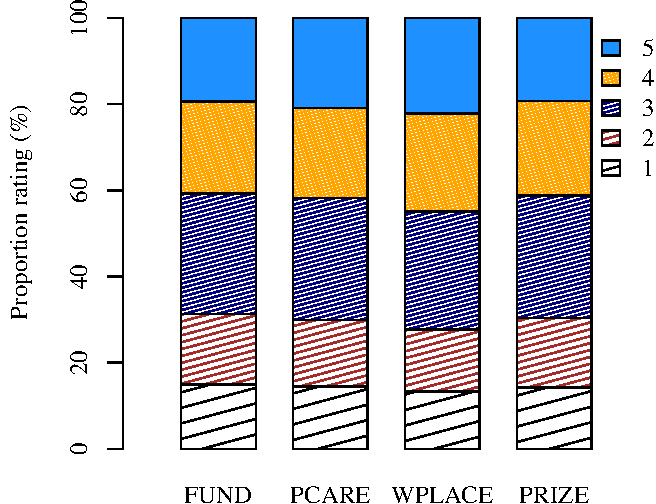
\includegraphics{figures/figure_ratings-1.pdf}
\end{figure}

The above analysis on the aggregate ratings does not hold in
general.\footnote{It crucially relies on the assumption that an
  increment in a proposal's quality as measured by an increase in
  ratings from \(v\) to \(v+1\) is the same for any value \(v\).} So, we
also examine the distribution of ratings as generated by treatments with
no aggregation. We have over 12,000 ratings, providing a very sensitive
test for differences across treatments. Using a Pearson's Chi-squared
test we find that the hypothesis of dependence between the distribution
of ratings and the treatments is \emph{not} quite significant at the 10
percent level (p-value of 0.103). Driving the p-value is a less than
\(2\) percent difference between the proportion of 5's in the WPLACE
treatment versus the other distributions, which is probably due to
outliers (the winning proposal was in the WPLACE treatment). Taken
together with the fact that our sample is large, we have strong evidence
suggesting that there are no (economically meaningful) differences in
the quality of project proposals across treatments and in particular no
evidence of a quantity versus quality trade-off up to the resolution of
the five-point scale.\footnote{One may worry that such binning is a
  fairly coarse measure of quality. In particular, effects concentrated
  in the upper tail of the distribution may not be detected. For
  example, compare the ratings of proposals A, B, C and D with
  hypothetical true qualities of 3, 4, 5, and 10 stars respectively.
  Under a five-point scale rating system, proposals A and B can be
  distinguished, but C and D cannot be distinguished. Hence, one needs
  to be very cautious in interpreting these results as evidence against
  quality effects in general.}

\subsubsection{Quality assessed by
managers}\label{quality-assessed-by-managers}

One potential limit of assessing quality only on the basis of peer
ratings is that the employees might have a different view of a
proposal's quality than executives (due, for instance, to a misalignment
of incentives). Indeed, to ensure alignment between managerial goals and
the peer assessment, all project proposals were further vetted by the
HTL staff before being considered for implementation funding. So, we now
focus on the outcomes of this vetting process to investigate more
broadly the presence of treatment effects on the quality of project
proposals.

The vetting process conducted by the HTL staff resulted in 93 proposals
being scored (from 1 to 100 points) with the best 29 proposals invited
to submit implementation plans. The remaining 20 proposals were excluded
(and received a score of zero) either because flagged as inappropriate
for funding or because the proponent manifested no intention to
participate in the implementation phase (a Fisher's Exact Test for Count
Data finds no association between proposals excluded and treatments with
a p-value of 0.652).

The Spearman's rank correlation coefficient between the scores given by
the HTL staff and the average peer ratings was relatively high (0.198),
indicating good agreement between our two measures of quality. Indeed,
as before, we find no treatment effects on quality using the scores (a
Kruskal-Wallis rank sum test gives a p-value of 0.437). We also find no
treatment differences in the percentage of submitters being selected and
invited by HTL staff to present additional implementation plans (a
Fisher's Exact Test for Count Data gives a p-value of 0.652). Although
not significant, employees who made project proposals in the FUND
solicitation treatment are less likely to be selected as finalist than
the others (only 1 out of 7 in the FUND treatment were selected and
invited by the HTL staff), providing additional evidence of a no
quantity versus quality trade-off, as discussed before.

\subsection{The content of the project
proposals}\label{the-content-of-the-project-proposals}

The goal of the challenge was to improve Heart Center operations by
identifying problem areas and potential solutions. The proposed projects
broadly conformed to the stated goals of the contest, aligning with
improving the work processes within the organization or providing
high-quality patient care. For example, one project proposal that
received high peer ratings was to create a platform for patients to
electronically review and update their medicine list in the office prior
to seeing the physician. Another was to develop a smartphone application
showing a patient's itinerary for the day providing a guide from one
test or appointment to another. Nevertheless, other contest organizers
may have varying goals and be concerned about different aspects of the
submissions.

In order to examine additional dimensions of submission content, we now
study the area of focus of the submissions. Of particular interest is
understanding whether different wordings used in the general
encouragement solicitations (either towards improving the workplace or
targeting the wellbeing of patients) induce employees to concentrate on
different categories.

\begin{table}
\centering
\caption{Project proposals by area of focus}
\label{tab: area-of-focus}
\begin{tabular}{@{}lccccc}
  \\[-1.8ex]\hline \hline \\[-1.8ex]
 & FUND & PCARE & WPLACE & PRIZE & Total \\ 
  \hline \\[-1.86ex]
Information and access & 0 & 4 & 8 & 11 & 23 \\ 
  Patient support & 2 & 8 & 7 & 6 & 23 \\ 
  Care Coordination & 1 & 9 & 3 & 7 & 20 \\ 
  Staff workflow & 4 & 5 & 4 & 5 & 18 \\ 
  Workplace & 3 & 6 & 3 & 5 & 17 \\ 
  Quality and safety  & 0 & 0 & 5 & 5 & 10 \\ 
  Surgical tools and support to research & 1 & 1 & 0 & 0 & 2 \\ 
  [1.8ex] Total & 11 & 33 & 30 & 39 & 113 \\ 
   \\[-1.8ex]\hline \hline \\[-1.8ex]
\end{tabular}
\begin{tablenotes}
The areas of focus were manually identified by executives at the end of the competition for all the project proposals (due to a technical problem five proposals ended up with no classification).
\end{tablenotes}
\end{table}

Members of the HTL categorized each project proposal into one of seven
``areas of focus'' (Table \ref{tab: area-of-focus}): three categories
(``Care coordination'', ``Staff workflow'', ``Workplace'') identified
improvements for the workplace, other three (``Information and access'',
``Patient care'', and ``Quality and Safety'') focused on improvements
centered around patients, and another one (``Surgical tools and support
to research'') categorized projects developing tools to support
scientific research.

We test overall association between these categories and the
solicitation treatments with a Fisher's Exact Test for Count Data with
simulated p-value (based on 50000 replicates). Results show a marginally
significant (p=0.088) association, which means that our solicitation
treatments have indeed an effect on the content of the submitted
proposals.

To test which areas of focus was affected by our treatment, we regress
the probability of a project proposal being in a given category against
solicitation treatment dummies. We use an F-test where the null
hypothesis tested is that all the treatment effects have a zero effect
on the probability of the proposal being in a given category. The
results of these F-tests of overall significance (Table
\ref{areas of focus}) reveals significant differences in the ``Quality
and Safety'' and ``Information and access'' categories, which we view as
improvements centered around patients (as opposed to workplace
improvements). The first significance result is due to project proposals
in the PCARE solicitation treatment being less likely to fall in the
``Quality and Safety'' category. The second result is due to project
proposals in the FUND solicitation treatment being less likely to fall
in the ``Information and access'' category.

Although it is difficult to interpret these results because our model
does not provide any prediction on the content of proposals, they
indicate a possible trade-off between stimulating participation via
solicitations and inducing selection in the type of contributions to the
public good, which complicates the analysis of incentives for public
goods inside organizations beyond what the current literature
anticipates.

\begin{table}
\centering
\caption{Areas of Focus and Solicitation Treatment}
\label{areas of focus}
\begin{tabular}{@{}lcc}
  \\[-1.8ex]\hline \hline \\[-1.8ex]
 & F value & Pr($>$F) \\ 
  \hline \\[-1.86ex]
Patient support & 0.357 & 0.784 \\ 
  Information and access & 2.185 & 0.094 \\ 
  Quality and safety  & 2.512 & 0.062 \\ 
  Workplace & 0.751 & 0.524 \\ 
  Staff workflow & 1.291 & 0.281 \\ 
  Care Coordination & 1.284 & 0.283 \\ 
  Surgical tools and support to research & 1.660 & 0.180 \\ 
   \\[-1.8ex]\hline \hline \\[-1.8ex]
\end{tabular}
\end{table}

We also look at differences in the underlying complexity of the project
proposal as captured by differences in the length (i.e., the word count)
of a submission. Submissions were below 200 words in most cases with
little differences between the treatments. Indeed, testing for a
significant linear regression relationship between the length of
submissions and treatment dummies returned an overall insignificant
result (p=.43, F-test).

As a result, based on the analysis of the areas of focus and the length
of the submissions, we do find only little evidence of differences in
submission content across treatments. However, submission content is not
a well-defined concept and could be characterized in many dimensions.
While content does not vary in the dimensions we selected, we have not
exhausted all possible dimensions.

\subsection{Estimating social
preferences}\label{estimating-social-preferences}

The analysis above has shown that our solicitation treatments had both
positive and negative effect on participation, with no effects on
quality, and little sorting based on gender or profession. But what can
we say about the employees' preferences towards the common goal of
improving the organization?

In this section, we calibrate the theoretical model developed in Section
\ref{analytical-framework-and-predictions} with the experimental data to
get a sense of the magnitude of underlying preferences for contributing
to the organization. Following, the mixed-strategy equilibrium of the
model, the theoretical probability of contributing must be proportional
to the expected value of winning, \(R\), the underlying preferences
towards the public good, \(\gamma\), the marginal costs of contributing,
\(c\), and the number of agents, \(n\).

We assume the cost of making a submission \(c\) is the same in each
treatment,\footnote{This seems a reasonable assumption, given everyone
  is asked to perform the same task (identical submission procedure,
  same word limit, etc.).} and the individual preferences are constant,
being predetermined to our intervention. Then we derive a structural
relationship between the observed difference in the probability of
contributing \(\Delta p\) and the difference in the expected rewards
from winning \(\Delta R\) between the treatments.That is,\footnote{This
  equation can be obtained by following these steps. First, we
  approximate the profit equating condition \eqref{eq: mixed-strategy}
  to a linear function by noticing that the \(1/(1-(1-p)^n)\)
  approximates one for \(n\) large enough and \(p\) sufficiently small.
  Second, we solve for \(p\) and we simplify using the definitions of
  \(\Delta p\) and \(\Delta R\).}

\begin{equation}
  \Delta p \approx\frac{\Delta R}{n (c - \gamma)}.
\end{equation}

(Throughout this section we will consider \(\delta=0\) ignoring the
distinction between impure and pure altruism.) By solving for
\(\gamma\), we get

\begin{equation}
  \label{eq: gamma}
  \gamma   \approx  c -  \Delta R / (n\Delta p). 
\end{equation}

This implies that the parameter capturing individual preference for the
public good (that is consistent with our data) must be proportional to
the ratio between the difference in rewards and the difference in the
probability of submitting. Although we do not observe the levels of
\(R\) in each treatment, we approximate the difference of rewards
between the PRIZE and the other conditions by the pecuniary value of the
reward, which has its upper bound in the highest price that can be paid
for an iPad mini (\$350).\footnote{The price paid by the Heart Center
  was \$239 at the end of 2014 (including shipping cost). Other popular
  models (those with cellular data and large storage) could cost as high
  as \$350. Agents, however, were not aware of the specific model used
  for the competition and of the price paid. So, the value of \$350 is
  very conservative.} We further calibrate the cost of submitting a
proposal \(c\) to \$40 which is the median income per hour of a Nurse
Practitioner according to the Bureau of Labor Statistics; we assume the
number of competitors \(n\) to be 30 percent of the entire sample to
take into account rational expectations about the actual number of
participants in the contest.\footnote{This choice is our best guess of
  the number of active staff members at the Heart Center and is based on
  the number of employees who voluntarily took a survey before the
  experiment (378 people). Assuming greater participation would lead to
  artificially increasing the estimates of underlying incentives. In
  fact, staff members may have rational expectations about the actual
  number of potential participants, which may be less than the entire
  population.} Finally, by substituting these calibrated values into
equation \eqref{eq: gamma} along with the empirical difference in
participation rates between the PRIZE and the other treatments
(\(\Delta p=0.037\)), we get an estimate of the magnitude of the social
preferences towards the organization which is \(\hat\gamma=\$12\). As
shown in Figure \ref{fig: gamma}, this value is equivalent to about 30
percent reduction in the cost of contributing. Hence, increasing the
prize by \$100 is expected to raise the probability of submitting by 1
percentage points. This increase can be compared to the corresponding
increase of 0.7 that one will obtain by assuming no social preferences
\(\gamma=0\) at all.

\begin{figure} 
\centering
\caption{Estimated value of social preferences ($\hat\gamma$)}
\label{fig: gamma}
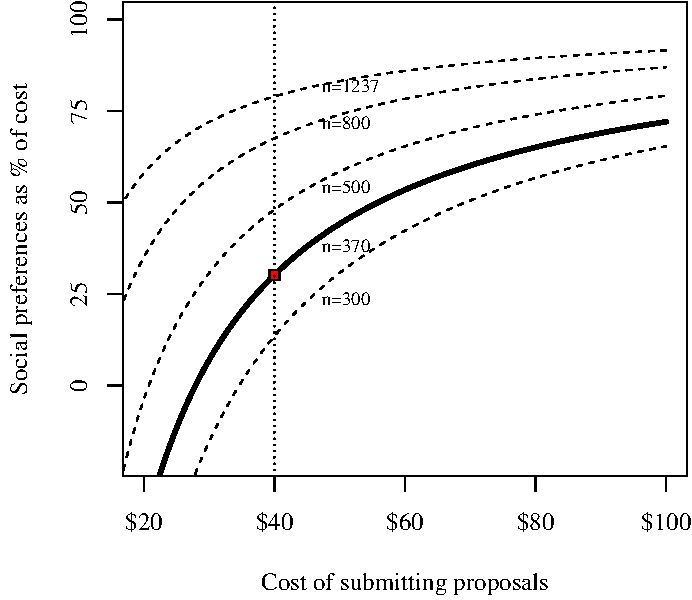
\includegraphics{figures/gamma-1.pdf}
\begin{tablenotes}
This figure plots the theoretical relationship between the cost of participation and the the social preferences parameter $\gamma$ (in percentage of the costs) which is consistent with our experimental data. Different curves represents different assumptions on the number of competitors. 
\end{tablenotes}
\end{figure}

A few remarks are in order here. To get confidence around these
estimates one need to consider several sources of uncertainty. First,
there is the uncertainty of estimating the probability of submitting in
our sample (standard errors can be computed directly from the data).
Another source of uncertainty is due to the calibration of the marginal
cost or the number of competitors. As shown in Figure \ref{fig: gamma},
the fraction of costs explained by social preferences increases
monotonically in the number of competitors (going up to 80 percent of
costs if employees expected to compete against every Heart Center staff
member); and decreases monotonically in the calibrated cost of making a
submission. Finally, another important source of uncertainty is
regarding the main behavioral assumptions of the model, as we discuss in
the next section.

\renewcommand\refname{References}
\bibliography{refs.bib}

\end{document}